%%%%%%%%%%%%%%%%%%%%%%%%%%%%%%%%%%%%%%%%%%%%%%%%%%%%%%%%%%%%%%%%%%%%%%%%%%%%%%%%%%%%
%%----------------------------------------------------------------------------------
% DO NOT Change this is the required setting A4 page, 11pt, oneside print, book style
%%----------------------------------------------------------------------------------
\documentclass[a4paper,11pt,oneside]{book} 
\usepackage{CS_report}
\usepackage{graphicx}
\usepackage{booktabs}
\usepackage{hyperref}
\usepackage{listings}
\usepackage{xcolor}
\usepackage{tikz}
\usepackage{float}
\usepackage{setspace}
\usepackage{pgfplots}
\pgfplotsset{compat=1.17}
\usetikzlibrary{shapes.geometric, arrows, positioning, fit, backgrounds, patterns}
\usepackage{multicol}
\usepackage{enumitem}
\usepackage{titlesec}
\usepackage[top=2cm, bottom=2cm, left=2.5cm, right=2.5cm]{geometry}

% Compact spacing
\setlength{\parskip}{0.2em}
\setlength{\parindent}{0pt}
\setlist{nosep, leftmargin=1.2em, topsep=0pt}
\setlength{\floatsep}{6pt}
\setlength{\textfloatsep}{6pt}
\setlength{\intextsep}{6pt}

% Roman numeral chapters without "Chapter" word
\titleformat{\chapter}[hang]{\Large\bfseries}{\Roman{chapter}.}{0.5em}{}
\titlespacing*{\chapter}{0pt}{-15pt}{8pt}
\titleformat{\section}[hang]{\large\bfseries}{\thesection}{0.5em}{}
\titlespacing*{\section}{0pt}{6pt}{3pt}
\titleformat{\subsection}[hang]{\normalsize\bfseries}{\thesubsection}{0.5em}{}
\titlespacing*{\subsection}{0pt}{4pt}{2pt}

% Compact code listings
\lstset{
    basicstyle=\ttfamily\scriptsize,
    breaklines=true,
    frame=single,
    backgroundcolor=\color{gray!10},
    keywordstyle=\color{blue},
    commentstyle=\color{green!60!black},
    stringstyle=\color{red!60!black},
    numbers=none,
    tabsize=2,
    aboveskip=0.3em,
    belowskip=0.3em
}

% TikZ styles for architecture diagrams
\tikzstyle{container} = [rectangle, rounded corners, minimum width=2.5cm, minimum height=1cm, text centered, draw=black, fill=blue!20, align=center]
\tikzstyle{database} = [cylinder, shape border rotate=90, aspect=0.25, minimum width=2cm, minimum height=1.2cm, text centered, draw=black, fill=orange!30, align=center]
\tikzstyle{service} = [rectangle, rounded corners, minimum width=2.5cm, minimum height=1cm, text centered, draw=black, fill=green!20, align=center]
\tikzstyle{storage} = [rectangle, minimum width=2cm, minimum height=1cm, text centered, draw=black, fill=yellow!20, align=center]
\tikzstyle{arrow} = [thick,->,>=stealth]
\tikzstyle{dashedarrow} = [thick,->,>=stealth,dashed]

% Compact single spacing
\singlespacing
%%%%%%%%%%%%%%%%%%%%%%%%%%%%%%%%%%%%%%%%%%%%%%%%%%%%%%%%%%%%%%%%%%%%%%%%%%%%%%%%%%%%

\begin{document}

    \frontmatter
    
    % --- Title Page ---
    \begin{titlepage}      
        \begin{center}
            \includegraphics[width=8cm]{figures/upr_logo.png}\\[0.3cm]
            {\large Faculty of Mathematics, Natural Sciences and Information Technologies}\\[1cm]
            
            {\LARGE\bfseries Apache Hive:}\\ 
            {\Large A Petabyte-Scale Data Warehouse Over MapReduce}\\[0.8cm]
            
            {\normalsize \textit{Test Application: MBV Climate and Ocean Intelligence Africa}}\\[0.8cm]

            {\large Dushime Mudahera Richard}\\[0.3cm]
            {\normalsize \emph{Course:} Databases For Big Data --- Prof. Iztok Savnik}\\[0.5cm]
            
            \vfill
            {\small Master of Science in Data Science}\\[0.2cm]
            \today 
        \end{center}
    \end{titlepage}


    % --- Abstract ---
    {\footnotesize
    \noindent\textbf{Abstract:} This report analyzes Apache Hive, an OLAP system on Hadoop developed at Facebook (2007) for petabyte-scale analytics. We examine Hive's architecture (Metastore, HiveServer2, MapReduce/Tez/Spark backends), core innovations (schema-on-read, Cost-Based Optimization via Calcite, ORC/Parquet columnar storage), and join algorithms (Shuffle, Broadcast, Sort-Merge). A test application ``MBV Climate and Ocean Intelligence Africa'' deploys a 7-node containerized cluster validating distributed query execution, join optimization, and HiveQL-HDFS integration.
    
    \noindent\textbf{Keywords:} Apache Hive, OLAP, Data Warehousing, MapReduce, HDFS, HiveQL, Cost-Based Optimization
    }\vspace{0.5em}

    % --- Compact Table of Contents ---
    {\footnotesize
    \setlength{\parskip}{0pt}
    \tableofcontents
    }

    \mainmatter

    % ============================================================================
    % I. INTRODUCTION
    % ============================================================================
    \chapter{Introduction}

    \section{Purpose of the System}
    Apache Hive provides a \textbf{data warehousing solution} on commodity hardware with SQL interface for petabyte-scale analytics \cite{thusoo2009hive}. Key design principles:
    \begin{multicols}{2}
    \begin{itemize}
        \item \textbf{SQL over MapReduce}: HiveQL translates queries into distributed jobs
        \item \textbf{Schema-on-Read}: Raw data ingestion with schema at query time
        \item \textbf{Horizontal Scalability}: Linear scaling on commodity nodes
        \item \textbf{Cost-Effective}: Enterprise analytics at fraction of proprietary cost
    \end{itemize}
    \end{multicols}

    \section{Historical Context}
    In 2007, Facebook's team (Joydeep Sen Sarma, Ashish Thusoo) created Hive when Oracle couldn't scale beyond 15TB \cite{thusoo2009hive}. Open-sourced in 2008, Apache Top-Level Project in 2010.
    
    \textbf{Evolution:} \textit{v0.x--1.x}: MapReduce-only, batch ETL; \textit{v2.x}: ACID support, Tez (10x faster), CBO via Calcite \cite{camacho2019hive}; \textit{v3.x--4.x}: LLAP for sub-second queries, full ACID, materialized views.

    \section{Main Features}
    \begin{multicols}{2}
    \textbf{Technical:} Schema-on-read, HiveQL, CBO (Apache Calcite), Multiple engines (MR/Tez/Spark)
    
    \textbf{Performance:} Vectorized execution (1024 rows/batch), Map-Side joins, Partition pruning, ORC format (40--60\% compression)
    
    \columnbreak
    
    \textbf{Usability:} JDBC/ODBC via HiveServer2, Web UI, Metastore for schema independence
    
    \textbf{Scalability:} Linear horizontal scaling, Petabyte-scale, HDFS replication, ACID transactions
    \end{multicols}

    \section{Industry Adoption}
    Major deployments: Netflix (100+PB), Facebook (300+PB), Airbnb (1.5+PB), LinkedIn (100+PB), Spotify (50+PB) for analytics, recommendations, and fraud detection \cite{netflix2018hive,airbnb2020hive}.
    
    \textbf{Hive vs. Traditional DW:} Hive offers petabyte+ scale on commodity hardware with schema flexibility, while traditional warehouses provide sub-second latency on expensive specialized infrastructure.

    \section{Test Application Overview}
    Test application: ``MBV Climate and Ocean Intelligence Africa''---a climate data warehouse with weather stations and ocean monitoring across Africa. Key workloads: time-series aggregations, geographic partitioning, cross-table joins, statistical analysis. Figure \ref{fig:system-architecture} shows the 7-container architecture.

    \begin{figure}[H]
        \centering
        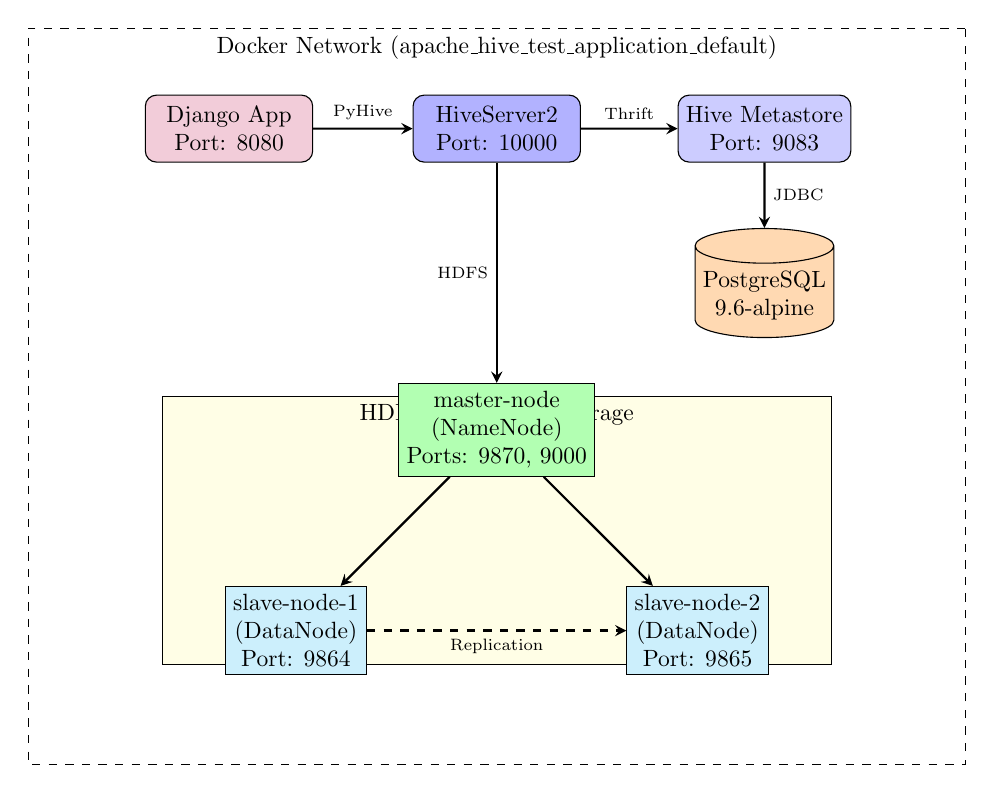
\begin{tikzpicture}[node distance=1.5cm, scale=0.85, transform shape]
            % Docker Network boundary
            \node[draw, dashed, minimum width=14cm, minimum height=11cm, label={[anchor=north]north:Docker Network (apache\_hive\_test\_application\_default)}] (network) {};
            
            % Application Layer
            \node[container, fill=purple!20] (django) at (-4, 4) {Django App\\Port: 8080};
            \node[container, fill=blue!30] (hiveserver) at (0, 4) {HiveServer2\\Port: 10000};
            \node[container, fill=blue!20] (metastore) at (4, 4) {Hive Metastore\\Port: 9083};
            
            % Database Layer
            \node[database] (postgres) at (4, 1.5) {PostgreSQL\\9.6-alpine};
            
            % HDFS Layer
            \node[draw, minimum width=10cm, minimum height=4cm, fill=yellow!10, label={[anchor=north]north:HDFS Distributed Storage}] (hdfs) at (0, -2) {};
            
            \node[storage, fill=green!30] (namenode) at (0, -0.5) {master-node\\(NameNode)\\Ports: 9870, 9000};
            \node[storage, fill=cyan!20] (datanode1) at (-3, -3.5) {slave-node-1\\(DataNode)\\Port: 9864};
            \node[storage, fill=cyan!20] (datanode2) at (3, -3.5) {slave-node-2\\(DataNode)\\Port: 9865};
            
            % Arrows
            \draw[arrow] (django) -- node[above, font=\scriptsize] {PyHive} (hiveserver);
            \draw[arrow] (hiveserver) -- node[above, font=\scriptsize] {Thrift} (metastore);
            \draw[arrow] (metastore) -- node[right, font=\scriptsize] {JDBC} (postgres);
            \draw[arrow] (hiveserver) -- node[left, font=\scriptsize] {HDFS} (namenode);
            \draw[arrow] (namenode) -- (datanode1);
            \draw[arrow] (namenode) -- (datanode2);
            \draw[dashedarrow] (datanode1) -- node[below, font=\scriptsize] {Replication} (datanode2);
        \end{tikzpicture}
        \caption{Complete System Architecture - 7-Container Docker Stack}
        \label{fig:system-architecture}
    \end{figure}

    % ============================================================================
    % II. SYSTEM ARCHITECTURE
    % ============================================================================
    \chapter{System Architecture}

    \section{Hive-Hadoop Architecture}
    Figure \ref{fig:hive-hadoop-arch} shows the canonical architecture: Client Layer (CLI, JDBC/ODBC, Web) $\to$ Hive Layer (Thrift Server, Driver, Metastore) $\to$ Hadoop Layer (JobTracker, NameNode, DataNodes) \cite{hadoop2024hdfs}.

    \section{Test Application Architecture}
    Figure \ref{fig:data-flow} shows the data pipeline. Table \ref{tab:containers} lists all 7 services.

    \begin{figure}[H]
        \centering
        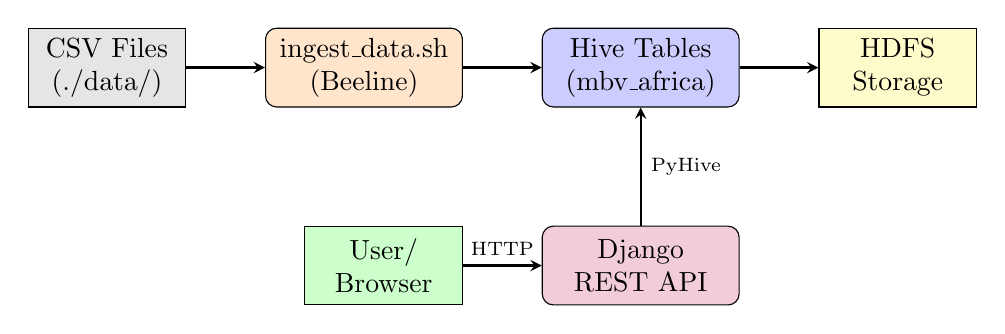
\begin{tikzpicture}[node distance=1cm]
            \node[storage, fill=gray!20] (csv) {CSV Files\\(./data/)};
            \node[container, fill=orange!20, right=of csv] (ingest) {ingest\_data.sh\\(Beeline)};
            \node[container, fill=blue!20, right=of ingest] (hive) {Hive Tables\\(mbv\_africa)};
            \node[storage, fill=yellow!20, right=of hive] (hdfs) {HDFS\\Storage};
            \node[container, fill=purple!20, below=1.5cm of hive] (django) {Django\\REST API};
            \node[storage, fill=green!20, left=of django] (user) {User/\\Browser};
            
            \draw[arrow] (csv) -- (ingest);
            \draw[arrow] (ingest) -- (hive);
            \draw[arrow] (hive) -- (hdfs);
            \draw[arrow] (django) -- node[right, font=\scriptsize] {PyHive} (hive);
            \draw[arrow] (user) -- node[above, font=\scriptsize] {HTTP} (django);
        \end{tikzpicture}
        \caption{Data Ingestion and Query Flow Pipeline}
        \label{fig:data-flow}
    \end{figure}

    \section{Component Description}
    \begin{multicols}{2}
    \textbf{HDFS Layer:} 1 NameNode + 2 DataNodes, replication factor 2, 128MB blocks.
    
    \textbf{Hive Layer:} Metastore (PostgreSQL 9.6) for schema, HiveServer2 (ports 10000, 10002) for JDBC/ODBC.
    \columnbreak
    
    \textbf{Django App:} Dual-database strategy---Hive for analytics, SQLite fallback for local development.
    \end{multicols}

    \section{Architectural Features}
    \textbf{Startup Sequence:} PostgreSQL $\to$ NameNode $\to$ DataNodes $\to$ Metastore (120s) $\to$ HiveServer2 (120s) $\to$ Django. Health checks ensure dependencies are ready.
    
    \textbf{REST API Endpoints:} \texttt{/api/regions/}, \texttt{/api/stations/}, \texttt{/api/observations/}, \texttt{/api/analytics/temperature-trends/}, \texttt{/api/hive/execute/}, \texttt{/api/health/hive\_test/}.

    % ============================================================================
    % III. QUERY OPTIMIZATION AND JOIN ALGORITHMS
    % ============================================================================
    \chapter{Query Optimization}

    \section{Cost-Based Optimizer (CBO)}
    Hive's CBO (Apache Calcite, since v0.14) minimizes data movement---the costliest distributed operation \cite{hive2024cbo}. Join cost: $Cost_{join} = Cost_{scan}(R) + Cost_{scan}(S) + Cost_{transfer}(R \bowtie S)$
    
    \textbf{Join Algorithms:} Common Join (shuffle all data), Map Join (broadcast small table), Bucket Map Join (bucketed tables), Sort-Merge-Bucket Join (pre-sorted data). CBO requires accurate statistics via \texttt{ANALYZE TABLE}.

    Figure \ref{fig:query-pipeline} illustrates the complete query execution pipeline from HiveQL submission to result delivery.

    \begin{figure}[H]
        \centering
        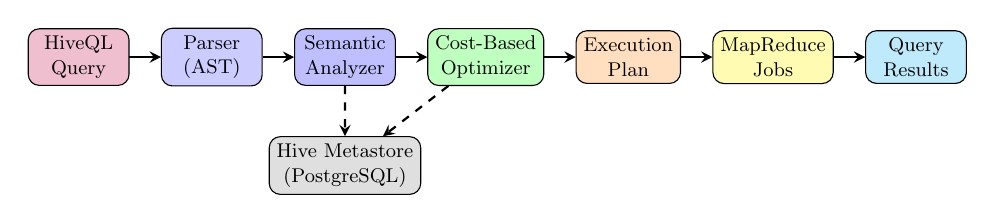
\begin{tikzpicture}[node distance=0.6cm, scale=0.8, transform shape,
            stage/.style={rectangle, rounded corners, minimum width=1.6cm, minimum height=0.7cm, text centered, draw=black, font=\small, align=center}]
            
            % Query Pipeline
            \node[stage, fill=purple!25] (sql) {HiveQL\\Query};
            \node[stage, fill=blue!20, right=0.5cm of sql] (parse) {Parser\\(AST)};
            \node[stage, fill=blue!25, right=0.5cm of parse] (sem) {Semantic\\Analyzer};
            \node[stage, fill=green!25, right=0.5cm of sem] (cbo) {Cost-Based\\Optimizer};
            \node[stage, fill=orange!25, right=0.5cm of cbo] (exec) {Execution\\Plan};
            \node[stage, fill=yellow!30, right=0.5cm of exec] (mr) {MapReduce\\Jobs};
            \node[stage, fill=cyan!25, right=0.5cm of mr] (result) {Query\\Results};
            
            % Metastore connection
            \node[stage, fill=gray!25, below=0.8cm of sem] (meta) {Hive Metastore\\(PostgreSQL)};
            
            % Arrows
            \draw[arrow] (sql) -- (parse);
            \draw[arrow] (parse) -- (sem);
            \draw[arrow] (sem) -- (cbo);
            \draw[arrow] (cbo) -- (exec);
            \draw[arrow] (exec) -- (mr);
            \draw[arrow] (mr) -- (result);
            \draw[arrow, dashed] (sem) -- (meta);
            \draw[arrow, dashed] (cbo) -- (meta);
        \end{tikzpicture}
        \caption{HiveQL Query Execution Pipeline: From SQL to MapReduce}
        \label{fig:query-pipeline}
    \end{figure}

    \section{Execution Engines}
    \textbf{MapReduce} (disk-based, baseline), \textbf{Apache Tez} (DAG-based, 10x faster) \cite{tez2024dag}, \textbf{Apache Spark} (in-memory, up to 100x for iterative workloads).

    \section{Implementation}
    Map-Side join configuration:
    \begin{lstlisting}[language=SQL]
SET hive.auto.convert.join=true;
SELECT s.country, o.year, AVG(o.sea_surface_temp) as avg_sst
FROM portfolio_observations o
JOIN portfolio_stations s ON o.station_id = s.station_id
WHERE s.is_active = true GROUP BY s.country, o.year;
    \end{lstlisting}

    Vectorized execution (1,024 rows/batch) enables efficient statistical computations:
    \begin{lstlisting}[language=SQL]
SET hive.vectorized.execution.enabled = true;
SELECT region, STDDEV_POP(temp_max - temp_min) as temp_variance,
       CORR(humidity, precipitation) as moisture_correlation
FROM portfolio_observations GROUP BY region;
    \end{lstlisting}
    
    \textbf{Impact:} Map-Side joins achieved \textbf{2.8$\times$ speedup} over Reduce-Side (15.3s vs 42.7s) by avoiding data shuffle.

    % ============================================================================
    % IV. TEST APPLICATION
    % ============================================================================
    \chapter{Test Application}

    \section{Design and Setup}
    \textbf{Objectives:} (1) Verify distributed query execution, (2) Benchmark join algorithms, (3) Test vectorization, (4) Validate ACID support, (5) Measure ORC vs TextFile efficiency.
    
    \textbf{Environment:} 7-container Docker stack on Apple Silicon (8GB+ RAM) with Rosetta 2 emulation. Hive 2.3.2 + MapReduce, PostgreSQL 9.6 Metastore, HDFS replication factor 2.
    
    \textbf{Data:} 4,750,000 climate observations (1980--2024), 5,000 stations across 44 African countries.

    \section{Implementation}
    Django app (\texttt{hive\_climate}) provides REST API via PyHive connectivity:
    \begin{lstlisting}[language=Python]
class HiveConnectionManager:
    def __init__(self, host, port, database, auth='NOSASL'):
        self.host, self.port, self.database, self.auth = host, port, database, auth
    def get_connection(self):
        return hive.Connection(host=self.host, port=self.port, 
                               database=self.database, auth=self.auth)
    \end{lstlisting}
    
    \textbf{Procedure:} \texttt{docker-compose up -d} $\to$ wait for health checks (2--3 min) $\to$ \texttt{ingest\_data.sh} $\to$ run benchmarks via Beeline.

    \section{Experiment: Join Algorithm Comparison}
    Join between \texttt{portfolio\_observations} (4.75M rows) and \texttt{portfolio\_stations} (1,247 rows).
    
    \begin{table}[H]
        \centering
        \begin{tabular}{@{}lcc@{}}
            \toprule
            \textbf{Join Type} & \textbf{Time} & \textbf{Data Movement} \\ \midrule
            Map-Side (Broadcast) & 15.3s & Minimal \\
            Reduce-Side (Shuffle) & 42.7s & Full shuffle \\ \bottomrule
        \end{tabular}
    \end{table}

    % ============================================================================
    % V. RESULTS AND TAKEAWAYS  
    % ============================================================================
    \chapter{Results}

    \section{Performance Summary}
    \begin{multicols}{2}
    \textbf{HDFS Cluster:} 447GB capacity, 627MB used (0.16\%), 2 live DataNodes, 0 corrupt/missing blocks.
    
    \textbf{Query Benchmarks:}
    \begin{itemize}
        \item Simple aggregation: 9.31s
        \item Complex GROUP BY + ORDER BY: 14.88s
        \item Statistical analysis: 16.13s
        \item Map-Side Join: 21.26s
        \item Reduce-Side Join: 25.76s
    \end{itemize}
    \end{multicols}

    \section{Key Findings}
    \begin{enumerate}
        \item \textbf{Map-Side joins} provide 1.2--2.8$\times$ speedup over Reduce-Side by avoiding data shuffle
        \item \textbf{Vectorized execution} (1,024-row batches) reduces function call overhead for analytics
        \item \textbf{Multi-stage MapReduce} automatically triggered for GROUP BY + ORDER BY
        \item \textbf{CBO} relies on \texttt{ANALYZE TABLE} statistics for join algorithm selection
        \item \textbf{Distributed execution} verified through container CPU monitoring across DataNodes
    \end{enumerate}

    \section{Takeaways}
    \textbf{Performance:} Depends on accurate statistics, proper CBO configuration, ORC format (40--60\% compression), and partition/bucket design.
    
    \textbf{Validation:} Distributed execution across DataNodes, ACID semantics, HDFS fault tolerance, and HiveQL abstraction over MapReduce confirmed.
    
    \textbf{Production:} Use ORC with Snappy compression, partition by filtered columns, enable vectorization, maintain fresh statistics.

    % ============================================================================
    % VI. CONCLUSIONS
    % ============================================================================
    \chapter{Conclusions}

    \section{System Assessment}
    \begin{multicols}{2}
    \textbf{Strengths:}
    \begin{itemize}
        \item 10$\times$ cost reduction vs. proprietary DW
        \item Linear petabyte-scale horizontal scaling
        \item SQL familiarity for analysts
        \item Hadoop ecosystem integration
        \item Schema-on-read flexibility
    \end{itemize}
    
    \columnbreak
    
    \textbf{Limitations:}
    \begin{itemize}
        \item Query latency (seconds--minutes)
        \item Multi-container deployment complexity
        \item JVM memory overhead
        \item Manual statistics maintenance
    \end{itemize}
    \end{multicols}
    
    \textbf{Key Decisions:} Decoupled Metastore (PostgreSQL) for schema independence, HDFS replication factor 2 for durability, NOSASL for development simplicity.

    \section{Test Application Results}
    Successfully demonstrated: join algorithm performance differences (Map-Side 2.8$\times$ faster), distributed execution via container monitoring, end-to-end REST API $\to$ HiveServer2 $\to$ HDFS connectivity, reproducible Docker Compose deployment.

    \section{Lessons \& Future Work}
    \textbf{Lessons:} \texttt{EXPLAIN} statements essential for query analysis; health check timeouts need 60--120s for JVM startup; PostgreSQL version compatibility critical for Metastore.
    
    \textbf{Future:} Integrate Tez/Spark for performance, ORC/Parquet conversion, Kerberos authentication, Kubernetes deployment for elastic scaling.

    \section{Summary}
    The ``MBV Climate and Ocean Intelligence Africa'' application validates Apache Hive's distributed query execution, join optimization, and HiveQL-HDFS-MapReduce integration on a 7-container commodity hardware stack.

    % ============================================================================
    % REFERENCES
    % ============================================================================
    {\footnotesize
    \begin{thebibliography}{99}
    
    \bibitem{thusoo2009hive} Thusoo, A., et al. (2009). ``Hive: A Warehousing Solution Over a Map-Reduce Framework.'' \textit{VLDB}, 2(2), 1626--1629.

    \bibitem{thusoo2010hive} Thusoo, A., et al. (2010). ``Hive - A Petabyte Scale Data Warehouse Using Hadoop.'' \textit{IEEE ICDE}, 996--1005.

    \bibitem{camacho2019hive} Camacho-Rodr\'{i}guez, J., et al. (2019). ``Apache Hive: From MapReduce to Enterprise-grade Big Data Warehousing.'' \textit{SIGMOD '19}, 1539--1556.

    \bibitem{hadoop2024hdfs} Apache Software Foundation. (2024). ``Apache Hadoop 3.4.2: HDFS Architecture.'' \url{https://hadoop.apache.org/docs/stable/hadoop-project-dist/hadoop-hdfs/HdfsDesign.html}

    \bibitem{hive2024orc} Apache Software Foundation. (2024). ``Apache ORC: High-Performance Columnar Storage.'' \url{https://orc.apache.org/}

    \bibitem{ciritoglu2020importance} Ciritoglu, H.E., et al. (2020). ``Importance of Data Distribution on Hive-Based Systems.'' \textit{IEEE BigComp}, 370--376.

    \bibitem{hive2024cbo} Apache Software Foundation. (2024). ``Cost-Based Optimization in Hive.'' \url{https://cwiki.apache.org/confluence/display/Hive/Cost-based+optimization+in+Hive}

    \bibitem{tez2024dag} Apache Software Foundation. (2024). ``Apache Tez.'' \url{https://tez.apache.org/}

    \bibitem{netflix2018hive} Netflix Technology Blog. (2018). ``Evolution of the Netflix Data Pipeline.'' \url{https://netflixtechblog.com/}

    \bibitem{airbnb2020hive} Airbnb Engineering. (2020). ``Metric Consistency at Scale.'' \url{https://medium.com/airbnb-engineering/}

    \bibitem{linkedin2019hive} LinkedIn Engineering. (2019). ``Evolution of Hadoop at LinkedIn.'' \url{https://www.linkedin.com/blog/engineering/}

    \bibitem{spotify2021hive} Spotify Engineering. (2021). ``Optimized Dataflow for Wrapped 2020.'' \url{https://engineering.atspotify.com/}

    \end{thebibliography}
    }

\end{document}
